\chapter{RTXI Features}

\marginlabel{Hard real-time platform} RTXI provides a platform for data acquisition and custom control paradigms involving a variety of hardware and software algorithms. It runs on a hard real-time Linux operating system (OS), which guarantees reliable timing for periodic tasks such as sampling from experimental equipment, performing computations, and generating external signals. This differs from platforms based on general purpose operating systems that assign different scheduling priorities to tasks based on optimizing the user experience in a multitasking environment. For closed-loop applications such as dynamic clamp that run at very high sampling rates, it is important that data is sampled at a precise time and that all computations are completed in time for the next scheduled feedback input. Operating systems that can absolutely guarantee a maximum time for these operations are referred to as �hard real-time,� while operating systems that can only guarantee a maximum most of the time are referred to as �soft real-time.� A soft real-time system can handle such lateness, usually by pausing processes with a lower priority. For dynamic clamp, a soft real-time system may occasionally wait so long to compute the injected current, that the actual value of the membrane potential has changed in the meantime. In that case, the simulated ion channel (or other membrane conductance) is based on incorrect assumptions about the state of the system. Real-time Linux also maximizes the sampling rate that can be used by minimizing system latencies related to the hardware and analog-to-digital conversion (and vice versa). For some experimental designs with closed-loop feedback, a higher sampling rate improves the stability of the protocol.

\marginlabel{Modular architecture}Users can quickly implement complex experimental protocols in RTXI, including both open and closed-loop control modes as well as many data acquisition modes. This is accomplished by RTXI's unique architecture in which system features and custom user code are implemented as modules. Modules contain function-specific code that can be used in combination to create larger workflows. They communicate with each other within the RTXI workspace by a system of  \emph{signals and slots} and event handling. All data acquired through a DAQ card are preserved as signal streams that can be passed to other modules that implement real-time analyses such as event detection, digital filters, etc. Similarly, all user modules can accept input signals and generate output signals that can be connected to other modules or to a DAQ card to produce external analog or digital signals. In the following example of a RTXI workflow for a dynamic clamp protocol, the recorded membrane potential from a cell is connected to a module that contains a model of an ion channel. The output of the module is the computed current, which is based on the value of Vm. The output signal from the ion channel module is connected to the DAQ card so that it can be injected back into the cell. The Oscillocope can plot any signal in the workspace, including actual outputs of a model as well as internally computed state variables.

\begin{figure}[h!]
\begin{maxipage}
\begin{center}
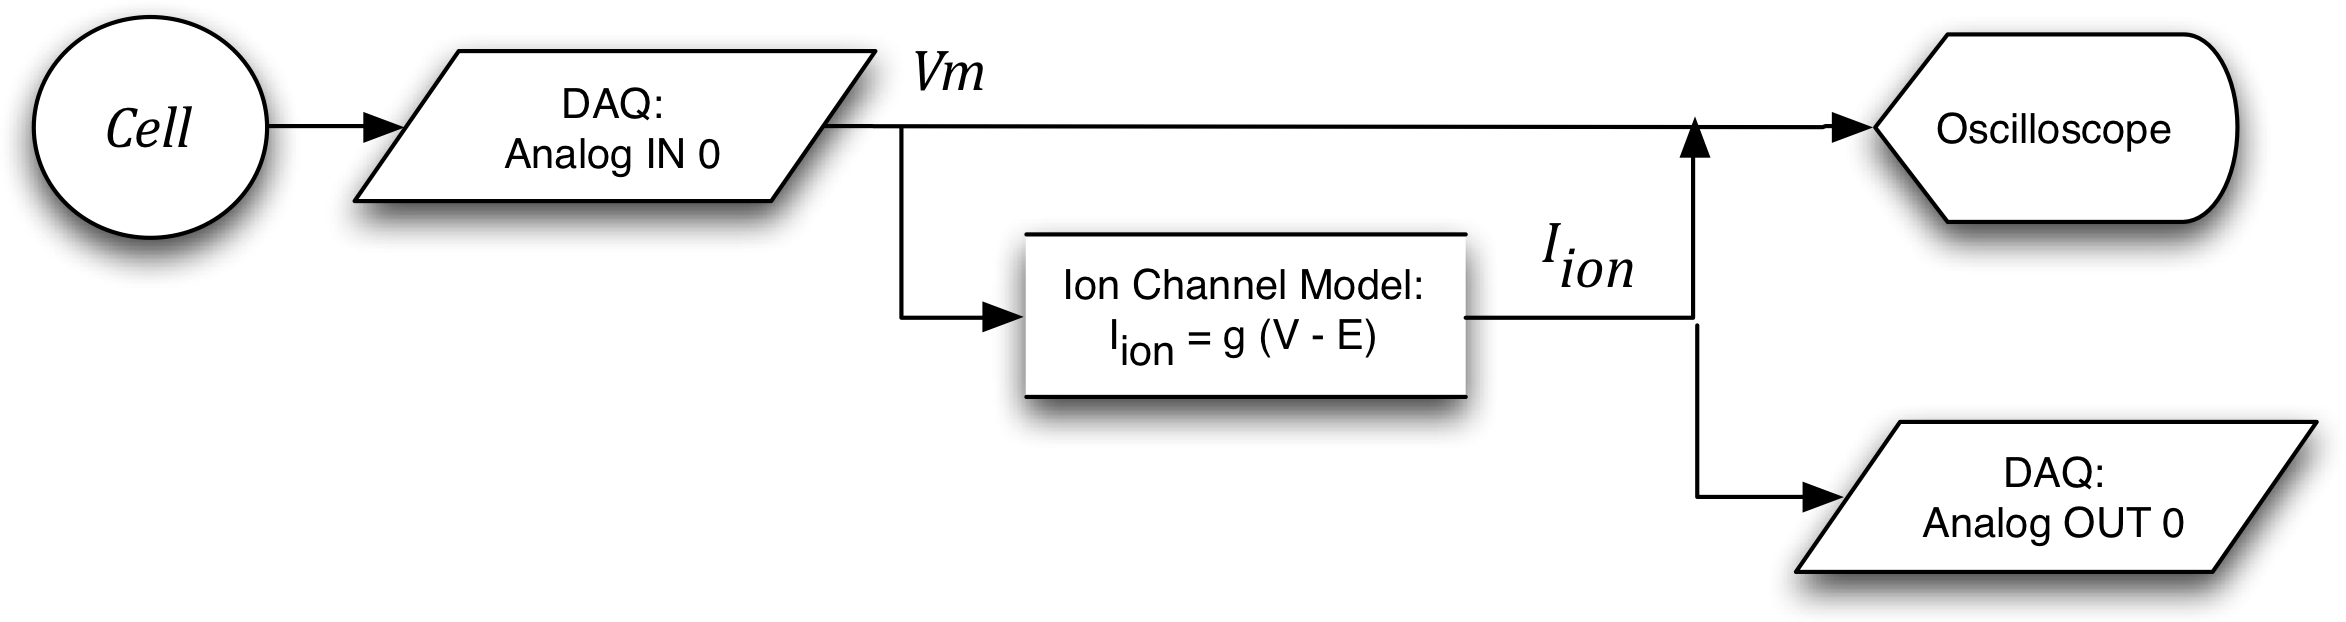
\includegraphics[width=6in]{module_ex1.png} 
\caption[RTXI Workflow Example 1]{A user module computes a current based on a model of an ion channel and the acquired value of the cell's membrane potential.} 
\label{fig:Workflow 1}
\end{center}
\end{maxipage}
\end{figure}

This modular signal-and-slots architecture allows multiple instantiations of user modules and all modules accept one-to-many and many-to-one connections. For example, a single module output signal can be routed to multiple targets. If multiple signals are connected to a single target, or slot, the signals are summed before being used in any further calculations within the module. This framework makes it easy to reuse code and implement branching logic. It is similar to graphical programming frameworks used in MATLAB\tm Simulink$^{\textrm{\textregistered}}$ and LabVIEW\tm. In the following example, a biological cell is reciprocally coupled through artificial synapses to a model neuron simulated within RTXI. The synapse is triggered by a presynaptic action potential and the synaptic current is modeled using a conductance-based equation that also depends on the measured membrane potential of the presynaptic neuron. In Figure \ref{fig: Workflow 2}, the membrane potential is split into two streams. One is sent to a Spike Detector module, which generates a trigger signal for the Synapse Model module. The other branch is sent directly to the Synapse Model module to be used in the calculation of the synaptic current. Each of these modules is instantiated twice since the two neurons are reciprocally coupled. Furthermore, each instantiation operates completely independently and can have different parameter values. This modular approach makes it very easy to experiment with asymmetric coupling, where one synapse is stronger than the other, by using different values for the maximal conductance or the reversal potential of the synapse.

This modular architecture also allows RTXI to be used solely as a experimental control system or as both a control system and data acquisition system. RTXI can be installed on most personal desktop and laptop computers and it is possible to run RTXI without a data acquisition card. This allows users to develop modules and online algorithms on one computer and copy their module to the actual computer used for experiments.

\begin{figure}[h!]
\begin{maxipage}
\begin{center}
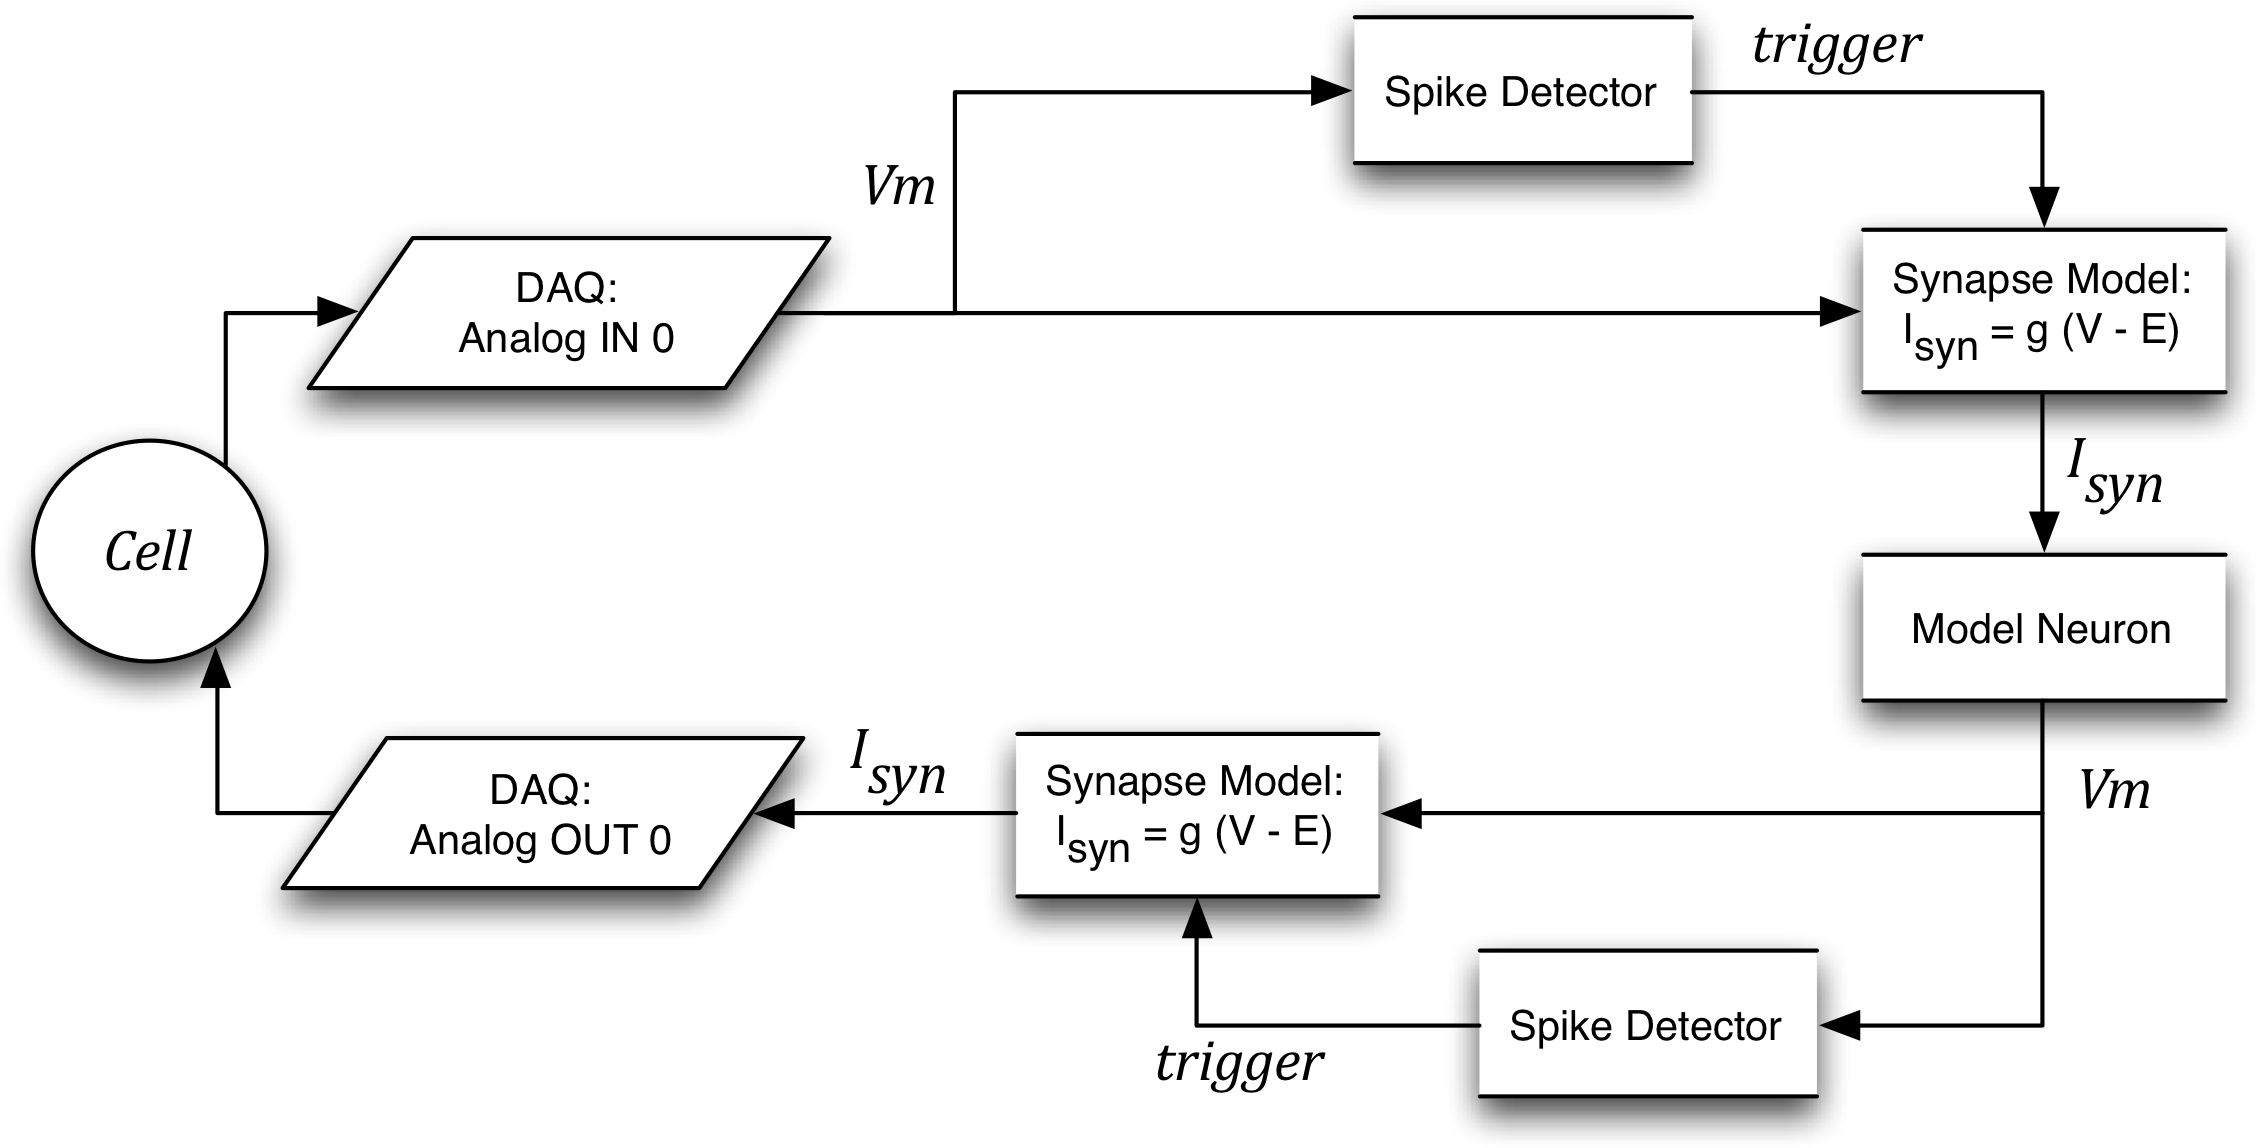
\includegraphics[width=6in]{module_ex2.png} 
\caption[RTXI Workflow Example 2]{Two user modules, a Spike Detector and a Synapse Model, are used to reciprocally couple a biological neuron with a model neuron. Each module is instantiated twice and can have different parameter values.} 
\label{fig: Workflow 2}
\end{center}
\end{maxipage}
\end{figure}

\marginlabel{Changing parameters on-the-fly} If you choose to change modules during an experiment, e.g. to change spike detection algorithms or use a different synaptic model, it is as simple as loading the new module and adding the connections. Other popular platforms for real-time closed-loop data acquisition may require you to recompile your program or re-download it onto a dedicated real-time processor. Similarly, an important feature of RTXI is the ability to change experimental parameters on-the-fly without recompiling or stopping real-time execution. This is accomplished through an intuitive GUI interface.

\marginlabel{Custom algorithms}RTXI and all core system features are written in \cpp and are based on the Qt GUI framework. Users implement custom experimental protocols by \seealso{Chapter \ref{custommodules}\\Custom User Modules}writing their own modules, in either \cpp or the DYNAMO scripting language. User-contributed modules are available on the website (http://www.rtxi.org) and examples are included in the RTXI source code. There is virtually no limit to what can be implemented in RTXI. Users can link to \cpp libraries of their own or that others have created to leverage complex computations or algorithms. Custom protocols can include not only unique online or real-time analysis but also unique experimental \emph{control} paradigms. Examples include the automation of protocols by automatically changing parameter values or using event detection to trigger a new sequence of experimental perturbations. 

The flexibility of RTXI through custom \cpp modules gives it features that are not common to other data acquisition systems, especially those for electrophysiology experiments. For example, RTXI is a complete simulation platform that can be used to solve systems of differential equations in real-time and integrate biological signals acquired in real-time with model systems. This was demonstrated in Figure \ref{Workflow 2}. Modules can also be written to load data from external files. RTXI has the ability to ``play back" this previously acquired data or surrogate data as if it were being acquired in real-time. This is accomplished by using a module that generates an output signal based on this surrogate data. Thus, online algorithms in development can be thoroughly tested and debugged using actual real-time execution without using the resources and time required for setting up an actual experiment. There are several advantages of this approach over simulating real-time computation offline using other platforms. First, it automatically takes into account the computing overhead associated with the actual RTXI system and gives a more accurate picture of your real-time performance. It also eliminates any redundant programming tasks involved with migrating code between platforms.

\marginlabel{Custom data acquisition}By default, RTXI runs \emph{continuous} protocols in that both the Data Recorder and digital Oscilloscopes modules act primarily as chart recorders. In addition, modules continuously execute their real-time code until they are paused. More complex sequences of operations can be accomplished by programming different operating modes within a single module. It is also possible to write a module that programmatically starts and stops other user modules. These "parent" or "controller" modules can be used to construct complex sequences or hierarchies of experimental stimuli. \emph{Sweep-based} or \emph{trial-based} recordings are implemented by a module that instructs the Data Recorder to increment trials. In addition, a module that generates a timed trigger signal can be used along with the trigger feature of the Oscilloscope to align recorded data in time. Examples of all these methods of implementing complex control paradigms are available.

\marginlabel{Metadata capture}RTXI can be used in parallel with your choice of data acquisition software. However, RTXI's ability to capture important metadata about an experiment is only present if it is also used for data acquisition. This is accomplished through the Data Recorder system module which streams the acquired data along with any computed signal to a Hierarchical Data Format (HDF5) file. HDF5 is an open data model that is increasingly popular for representing complex data, data relationships, and their associated metadata. In RTXI, any module that generates data that is being saved to HDF5 also has its parameters and parameter values stored in the same file. This includes not only acquired data, but also any computed intermediate signal, which is valuable for debugging algorithms offline. When a parameter value is modified on-the-fly during data acquisition, the new value and a timestamp for the modification is also saved. Other system parameters are also automatically saved to the HDF5 file so that important metadata is always adjacent to the actual experimental data. RTXI modules also exist for explicitly saving comments or creating custom experimental logs to capture any additional information. Such user modules can be used to standardize experimental logs by providing templates for information that the user is expected to supply or a finite set of options the user can choose from.

\marginlabel{Portability}Once a protocol has been created by making connections between modules and setting parameter values, the entire workspace can be captured to a settings file. Reloading this file will restore all system and user module settings, as well as the layout of the windows on the screen. This reduces the chances of errors when setting up a complicated experiment. These settings files can be transferred between different computers as long as the target computer contains the modules that were used. This is \seealso{Chapter \ref{COMEDIsupport}\\COMEDI support}independent of the actual experimental equipment that you use for data acquisition and/or current injection. RTXI uses the open source COMEDI drivers, which provides a generic interface to your choice of hardware. Users should check that they are using the correct hardware driver and configure their channel gains such that RTXI modules are receiving values in the correct units. The settings file uses a simple XML-based syntax and can be opened in any generic text editor to manually edit the default parameter values.

\seealso{Chapter \ref{HDF5}\\HDF5}HDF5 files are also compatible with many commercial and free software for a variety of platforms. There is no required proprietary software for viewing or analyzing data stored in RTXI-generated HDF5 files. Much of the available software also support editing data in place within the HDF5 file or appending new data to an existing file. This allows users to add associated data such as images, post-processed data, or additional notes.